\section{Simple distributed image reconstruction}\label{dist}
How do we distribute the major cycle. We need to distribute every step, Gridding, FFT and Deconvolution.

Gridding, Large number of input data. This needs to be distributed
We use the Image domain gridding introduces in section \ref{hypo:idg} and use it as the basis for the distributed gridding.

The FFT is generally not worth distributing, if we can keep all the data in memory. When the gridding is done, in our setup, the grid is small enough to keep in memory. (cite distributed fftw)

Deconvolution is also worth distributing. CLEAN depending on the observation is the second most time consuming step. But gridding tends to be easier to distribute, so in some observations it is the most time consuming step.
Split the image into patches and deconvolve each patch.
Sadly not possible, we need communication. how we communicate is important.

We use a distributed Gridding and a distributed deconvolution. Which leads us to the following architecture.

\begin{figure}[h]
	\centering
	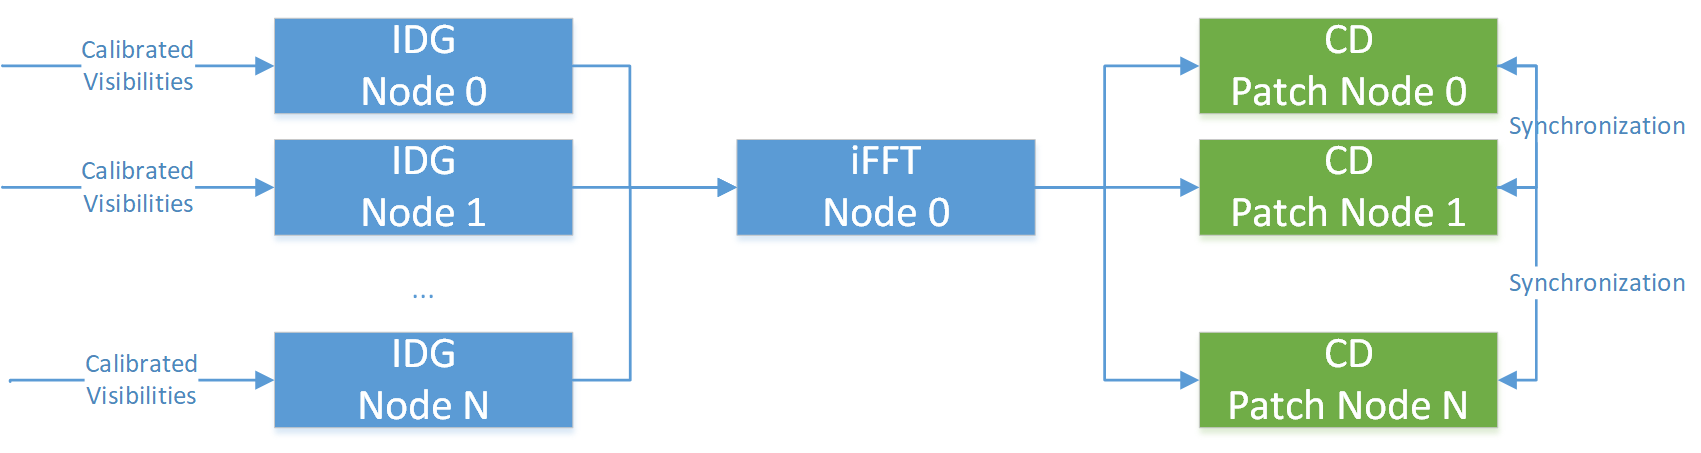
\includegraphics[width=0.80\linewidth]{./chapters/03.distribution/distributed_architecture.png}
	\caption{Distributed architecture for half a major cycle}
	\label{dist:architecture:fig}
\end{figure}

Where each node is one computer, i.e. has its own, possibly multiple cpus and its shared memory.
Split the input visibilities onto nodes. 
Do the gridding locally on each node
Communicate the grid
inverse FFT on one node.
Communicate the patches of the image.
Deconvolve each patch and communicate

How we distribute the IDG algorithm, and create a distributed deconvolution algorithm. Main contribution is the distributed deconvolution algorithm


\subsection{Distributing the IDG algorithm}\label{distribution:idg}




\subsection{Distributed deconvolution}

Main contribution
We start 

What we need: An optimization objective, an optimization algorithm and a regularization. 

We use \eqref{dist:deconv} as our optimization objective with data fidelity term and regularization term. We use Coordinate Descent Methods as our optimization algorithm, which we introduce in section \ref{dist:deconv:cd}, and the ElasticNet regularization, which we discuss in section \ref{dist:deconv:reg}

\begin{equation}\label{dist:deconv}
\underset{x}{minimize} \: \left \| I_{dirty} - x * PSF \right \|_2^2 + \lambda P(x)
\end{equation}



\subsubsection{Coordinate Descent Method}\label{dist:deconv:cd}
Coordinate Descent has gained more interest, because it may exploit sparse structures in the data.
Optimization for large data volume

Most problems become simple when we look at them in the one dimensional case. Finding the optimum to our objective \eqref{dist:deconv} is hard. But when we try to find the optimum of a single pixel, independent of all other pixels, the problem becomes simple. As we will see, we can find a closed form solution to find the optimum of a single pixel.
Coordinate Descent then optimizes a single pixel at a time, and we iterate over the whole image with some strategy until we converge. We may need to optimize the same pixel several times.

Monotone decreasing.
Robust
Many different variants.
How fast it is in practice depends on the regularization $P(x)$ we use.
Outperforms other algorithms like Gradient based methods, FISTA and ADMM if a single iteration (minimizing a single pixel in our case) is "cheap" to compute. 

\begin{lstlisting}
dirty = IFFT(Gridding(visibilities))
residuals = dirty

x = new Array
objectiveValue = SUM(residuals * residuals) + P(x)
oldObjectiveValue = objectiveValue

do 
{
	oldObjectiveValue = objectiveValue

	//the core of the algorithm
	pixelLocation = IterationStrategy(residuals)
	optimalValue = Minimize(residuals, pixelLocation)
	optimalValue = ApplyElasticNet(optimalValue)
	
	//housekeeping
	x[pixelLocation] = optimalValue
	residuals = (dirty - Convolve(x, psf))
	objectiveValue = SUM(residuals * residuals) + ElasticNet(x)
} while (oldObjectiveValue - objectiveValue)  < epsilon
\end{lstlisting}

The core of the algorithm consists of three functions: $ApplyElasticNet()$ which applies the closed form solution of the ElasticNet regularization (discussed in section \ref{dist:deconv:reg}), the $Minimize()$ function which minimizes a single pixel at a time and the iteration strategy. We derive a closed form solution for minimizing a single pixel independently of each other and then discuss the basics of the iteration strategy.

Let us derive the closed form solution to the $Minimize()$ function. We start by writing the data fidelity term as a quadratic equation: $(I_{dirty} - pixel * PSF)^2$, where $pixel$ is a scalar. Further, let us assume we only have a single pixel in the dirty image $I_{dirty}$ and a single pixel in the $PSF$. Everything is a scalar, it is easy to see that we are dealing with a parabola ($a*x^2 + b*x + c$. When we use our variable names we get $PSF^2 * pixel^2 - 2*(I_{dirty}*PSF)*pixel + (I_{dirty})^2$). We have a closed form solution to find the optimum of a parabola, i.e. $x_{opt} = \frac{-b}{2a}$, or when we use our variable names explicitly, we get $x_{opt} = \frac{(pixel*PSF)*I_{dirty}}{PSF^2}$. If we are dealing with more than one pixel in the dirty image $I_{dirty}$ and $PSF$, we multiply element-wise and sum up all the dimensions (i.e. $b = -2 SUM(pixel*PSF*I_{dirty})$). We found our closed form solution in the one dimensional case and we can implement $Minimize()$.

The next point is the iteration strategy. This is where Coordinate Descent methods are robust. They are proven to converge by simply choosing randomly. Or a greedy strategy where the pixel which reduces the objective \eqref{dist:deconv} by the largest amount. It was proven to converge for a variety of strategies. For this project, we are interested in which takes fewer computing resources to converge. 
Start with a greedy scheme, well known convergence guarantees at least linearly (with respect to iteration count?)\cite{luo1992convergence}
Cyclic scheme.

\subsubsection{Efficient Coordinate Descent implementation}\label{dist:deconv:efficient}
The question of efficient implementation. In the previous section, we have seen how coordinate descent works in general. But now we have to look at the details and see how we can implement it efficiently.

Question of convolution scheme. 
Circular convolution is physically not possible. The $PSF$ of the lower left corner does not wrap around the image and influence all other corners of the image. But as we will see, for an efficient coordinate descent we need to calculate a convolution to cache. The circular convolution is the output of the FFT. This is why reconstruction algorithms sometimes choose to use circular convolution \cite{ferrari2014distributed}.

The other convolution scheme, namely zero padding. We use this scheme. It results 

Iteration scheme. For a greedy iteration scheme, we would need to first:
\begin{enumerate}
	\item find the optimum pixel value for each pixel independently (i.e. $\frac{-b}{2a}$)
	\item evaluate which optimum pixel value results in the best reduction of the objective function \eqref{dist:deconv}
\end{enumerate}

For the first step, we can cache intermediate results and drastically reduce the computation. The second step can be approximated in a way that we do not need to evaluate the objective function.

\textbf{Caching intermediate results}\\
Caching of intermediate results. We have seen in section \ref{dist:deconv:cd} how we can find the optimum for a single pixel. We need to calculate  $x_{opt} = \frac{-b}{2a}$ where  $b = -2 SUM( pixel*PSF*I_{dirty})$ and $a = SUM(PSF * PSF)$. First, we note that $a$ depends only on the $PSF$ which is constant, which means $a$ is also constant. However, this is not true depending on the convolution we use.
$PSF$ at the corner gets masked off, and the $a$ value changes.
We can calucalte a lookup map in linear time.
\begin{lstlisting}

\end{lstlisting}

How to cache $b$. Use correlation of the dirty image with the $PSF$. Then we have a lookup map. Can be done efficiently in the Fourier domain. But the question then becomes in how to update bMap efficiently.


Unsolved problem of varying $PSF^2$

\textbf{Approximating the objective function}\\
$a$ is constant in $\frac{-b}{2a}$



Putting it all together. Creating lookup maps for $a$ and $b$, and do not evalue the ojbective function.
\begin{lstlisting}
dirty = IFFT(Gridding(visibilities))

//pre-calculate bMap
dirtyPadded = ZeroPadding(dirty, psfSize)
fourierDirtyPadded = FFT(dirtyPadded)
fourierPsf = FFT(invert(psf))		//we require the correlation, that is why we invert the psf
bMap = IFFT(fourierDirtyPadded * fourierPsf)

//pre-calculate aMap. aMap stays constant over all CD iterations
aMap = 
 
x = new Array   
do 
{
	oldObjectiveValue = objectiveValue
	
	//the core of the algorithm
	pixelLocation = IterationStrategy(residuals)
	optimalValue = Minimize(residuals, pixelLocation)
	optimalValue = ApplyElasticNet(optimalValue)
	
	//housekeeping
	x[pixelLocation] = optimalValue
	residuals = (dirty - Convolve(x, psf))
	objectiveValue = SUM(residuals * residuals) + ElasticNet(x)
} while (oldObjectiveValue - objectiveValue)  < epsilon
\end{lstlisting}



\subsubsection{ElasticNet Regularization} \label{dist:deconv:reg}
L2 norm was used in other work. \cite{ferrari2014distributed}

"Sparsifying L2 norm"
Remember the theory of compressed sensing.

Formula

\begin{figure}[h]
	\centering
	\begin{subfigure}[b]{0.3\linewidth}
		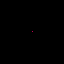
\includegraphics[width=\linewidth]{./chapters/03.distribution/L1.png}
		\caption{Effect of the pure L1 norm ($\lambda$ = 1.0) on a single point source.}
		\label{dist:cd:elastic:L1}
	\end{subfigure}
	\begin{subfigure}[b]{0.3\linewidth}
		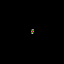
\includegraphics[width=\linewidth]{./chapters/03.distribution/L2.png}
		\caption{Effect of the pure L2 norm ($\lambda$ = 1.0) on a single point source.}
		\label{dist:cd:elastic:L2}
	\end{subfigure}
	
	\caption{Effect of the L1 and L2 Norm separately.}
	\label{dist:cd:elastic}
\end{figure}


Effect

Implementation, proximal operator. Shrinkage of a division.



May even speed up convergence for correlated pixel values compared to L1 or L2\cite{friedman2010regularization}. But was not investigated in this project

\subsection{Major Cycle convergence}
Putting it all together

We have the Minor Cycle, which is easy to converge.

Coordinate Descent Path optimization \cite{friedman2010regularization}
Danger that CD takes too many pixel into a Major Cycle. Lower bound per iteration, PSF sidelobe
  can still be too low, danger when many psf sidelobes overlap

\subsection{Test on MeerKAT data}

